\documentclass{article}
\usepackage{pgfplots}
\pgfplotsset{compat=1.17}

\begin{document}

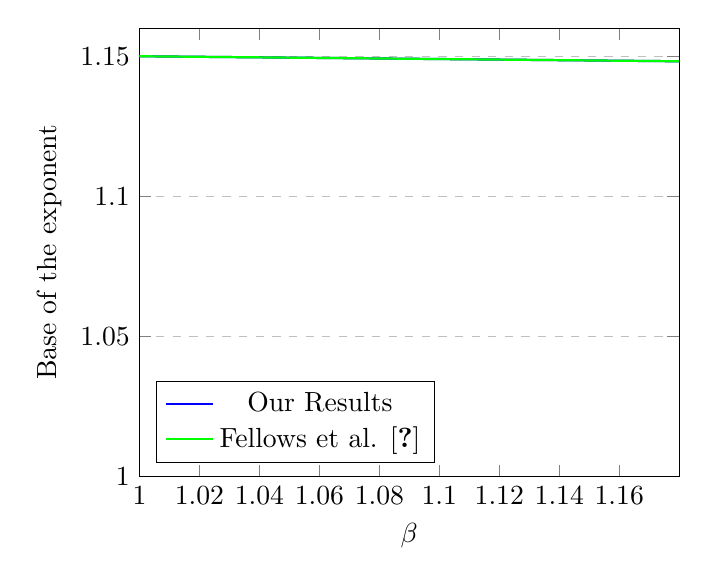
\begin{tikzpicture}
    \begin{axis}[
        xlabel={$\beta$},
        ylabel={Base of the exponent},
        xmin=1, xmax=1.18,
        ymin=1, ymax=1.16,
        xtick={1, 1.02, ..., 1.18},
        ytick={1, 1.05, ..., 1.16},
        legend pos=south west,
        ymajorgrids=true,
        grid style=dashed,
    ]
    
    % Our Results
    \addplot[
        domain=1:1.18,
        samples=200,
        color=blue,
        thick,
    ] {1.15 - 0.01 * (x - 1) + 0.0001 * (x - 1)^2};
    \addlegendentry{Our Results}
    
    % Fellows et al.
    \addplot[
        domain=1:1.18,
        samples=200,
        color=green,
        thick,
    ] {1.15 - 0.01 * (x - 1) + 0.0001 * (x - 1)^2};
    \addlegendentry{Fellows et al. \cite{fellows2004parameterized}};
    
    \end{axis}
\end{tikzpicture}

\caption{A plot of the running time of our algorithm for $\vcmaxdegthree$. The $x$-axis corresponds to the approximation ratio, while the $y$-axis corresponds to the base of the exponent in the running time. A point $(\beta, d)$ in the plot describes a running time of the form $d^{k} \cdot n^{\Oh(1)}$ for a $\beta$-approximation.}
\label{fig:running_time_plot}

\end{document}